%%%%%%%%%%%%%%%%%%%%%%%%%%%%%%%%%%%%%%%%%%%%%%%%%%%%%%%%%%%%%%%%%%%%%%%%%%%%%%%%
%2345678901234567890123456789012345678901234567890123456789012345678901234567890
%        1         2         3         4         5         6         7         8

\documentclass[journal]{IEEEtran}                         % Comment this line out
                                                          % if you need a4paper
%\documentclass[a4paper, 10pt, conference]{ieeeconf}      % Use this line for a4
            
\usepackage[utf8]{inputenc}                                        % paper

\overrideIEEEmargins
% See the \addtolength command later in the file to balance the column lengths
% on the last page of the document



% The following packages can be found on http:\\www.ctan.org
\usepackage{graphicx} % for pdf, bitmapped graphics files
\usepackage{bm}
\usepackage{blindtext}
\newcommand{\uvec}[1]{\boldsymbol{\hat{\textbf{#1}}}}
%\usepackage{epsfig} % for postscript graphics files
%\usepackage{mathptmx} % assumes new font selection scheme installed
%\usepackage{times} % assumes new font selection scheme installed
%\usepackage{amsmath} % assumes amsmath package installed
%\usepackage{amssymb}  % assumes amsmath package installed

\begin{document}
\markboth{This is my title and it really is a marvellous title, November~2019}%
{5G: The Next Step in Mobile Communications, November~2019}
\title{This is my title and it really is a marvellous title}


\author{Faris Nassif,~\IEEEmembership{Software Development (Honours),~GMIT}%
\thanks{}% <-this % stops a space
\thanks{$^{1}$Faris Nassif, G00347032, Software Development 2019}%
}

\maketitle


%%%%%%%%%%%%%%%%%%%%%%%%%%%%%%%%%%%%%%%%%%%%%%%%%%%%%%%%%%%%%%%%%%%%%%%%%%%%%%%%
\begin{abstract}

\blindtext 
 
\end{abstract}


%%%%%%%%%%%%%%%%%%%%%%%%%%%%%%%%%%%%%%%%%%%%%%%%%%%%%%%%%%%%%%%%%%%%%%%%%%%%%%%%
\section{INTRODUCTION}

\blindtext 
\blindtext 

\section{A Section}
Some of the various techniques being practiced worldwide are discussed below.


\subsection{A Subsection}
\blindtext 
\blindtext 
\blindtext 

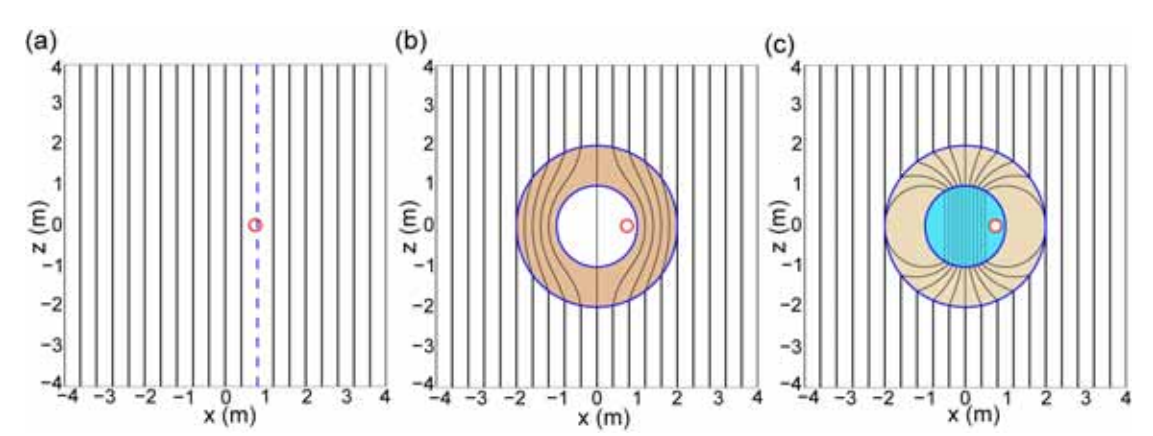
\includegraphics[scale=0.25]{1} 
\Blindtext 



\subsection{Another Subsection}
\blindtext 
\blindtext 


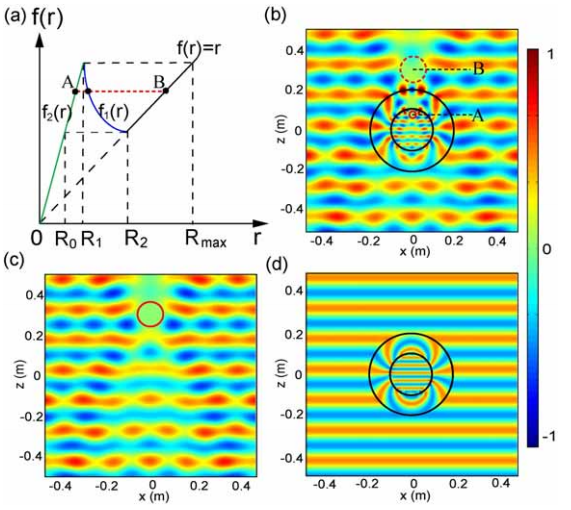
\includegraphics[scale=0.55]{2}

\blindtext 
\blindtext 


\subsection{A Subsection}
\blindtext 
\blindtext 


\subsection{Subsection}

\blindtext 



\section{ConclusionSection}
\blindtext 

     

\begin{thebibliography}{99}

\bibitem{c1} 1.	 Yan, M.; Ruan, Z.; Qiu, M. (2007). "Cylindrical Invisibility Cloak with Simplified Material Parameters is Inherently Visible".
\bibitem{c2} Ruan, Z.; Yan, M.; Neff, C. W.; Qiu, M. (2007). "Ideal Cylindrical Cloak: Perfect but Sensitive to Tiny Perturbations". 
\bibitem{c3}Greenleaf, A.; Kurylev, Y.; Lassas, M.; Uhlmann, G. (2007). "Improvement of cylindrical cloaking with the SHS lining".
\bibitem{c4} Yu Luo, Jingjing Zhang, Hongsheng Chen, Bae-Ian Wu, and Jin Au Kong(2007). "A new strategy to conceal an object from electromagnetic wave"





\end{thebibliography}




\end{document}
